\documentclass[12pt]{article}
\usepackage[T1]{fontenc} 
\usepackage[portuguese]{babel}
\usepackage{hyphenat}
% use se você precisar forçar a separação de sílabas em quebra de linha
\hyphenation{mate-mática recu-perar}
\usepackage{graphicx}
\graphicspath{images/}
\usepackage{csquotes}
\usepackage{subfiles}
\usepackage{amsmath}
\usepackage{csvsimple} 
\usepackage{geometry}

\geometry{
    a4paper,
    left=3cm,
    top = 3cm,
    right=2cm,
    bottom=2cm
}
\setlength{\parindent}{4em}
%\setlength{\parskip}{1em}
\renewcommand{\baselinestretch}{1.5}

\usepackage[dvipsnames]{xcolor}
\definecolor{alert}{RGB}{201, 58, 128}
\setlength {\marginparwidth }{2cm} 
\usepackage[colorinlistoftodos]{todonotes}
\usepackage{comment}
\usepackage{subcaption}
\DeclareUnicodeCharacter{0301}{*************************************}
\usepackage{enumitem}
%% CSS: mudando o gerenciador de bibliografia para biblatex para contornar 
% alguns problemas. Adendo: a compilação no overleaf ficou muito instável 
% e por alguma razão não imprime a seção de bibliografia no final, apesar
% de colocar as anotações ao longo do texto. Voltando ao bibtex no momento (5/9/2024)
%\usepackage{biblatex}
%\addbibresource{ref.bib}

%% TODO:
% - Resolver a questão com biblatex no overleaf
\title{TÍTULO}
\author{autor}

\begin{document}

% CAPA
\thispagestyle{empty}
    \begin{flushright}
        \begin{huge}
            \textbf{RELATÓRIO}\\[3,5cm]
        \end{huge}
%% CSS: Podemos usar um título mais genérico agora e depois discutir um definitivo
{\bf \LARGE  CLASSIFICAÇÃO DE GLAUCOMA EM IMAGENS DE FUNDO DE OLHO COM APRENDIZAGEM PROFUNDA}

\bigskip
        
        Leandro Zangirolami Trovões (Orientando)\\
        Carlos da Silva dos Santos (Orientador)\\
        Universidade Federal do ABC\\[5,5cm]
    \end{flushright}

    \vfill
    
    \begin{center}
        Santo André,\\
        Dezembro de 2024
    \end{center}
    
    \newpage
\bigskip

\begin{center}
\noindent{\bf \Large Resumo}
\end{center}

\begin{quote}
O glaucoma é a principal causa de cegueira irreversível no mundo, podendo atingir até 111,8 milhões de pessoas até 2040. Caracterizada pelo dano progressivo ao nervo ótico, a doença não tem cura e é assintomática em seus estágios iniciais, tornando o diagnóstico precoce essencial para retardar ou prevenir sua progressão. O exame de fundoscopia é uma das principais formas de identificar a doença, no qual é possível observar alterações características do glaucoma. Recentemente, técnicas de aprendizagem profunda têm sido aplicadas no diagnóstico de glaucoma em imagens de fundo de olho. O emprego de diferentes arquiteturas de redes neurais convolucionais tem apresentado resultados significativos. Contudo, a limitação da disponibilidade de imagens para treinamento e a falta de interpretabilidade são frequentemente apontadas como limitações.

Neste trabalho, apresentamos um modelo capaz de localizar o disco ótico em imagens de fundo de olho, baseado na arquitetura YOLO11 de rede neural convolucional. O modelo foi treinado com 1050 imagens do banco de dados JustRAIGS e atingiu precisão 0.999, recall 0.991 mAP50 0.995 e mAP50-95 0.934. Também apresentamos um modelo classificador preliminar para glaucoma, utilizando a arquitetura ResNet50. O modelo alcançou AUC-ROC 0,9789, PRC 0,9503, F1 0,9180, precisão 0,9060 e recall 0,9304.

\end{quote}

\begin{center}
Santo André, dezembro de 2024
\end{center}

\newpage
\bigskip

\section{Introdução}
\label{sec:introducao}

%% CSS: usar o ~ antes do \cite impede que o latex quebre linha entre 
% o texto e a anotação
% LZT: queremos evitar a quebra? Vi um caso em que a anotação chegou a
% passar da margem do documento para evitar a quebra.
Principal causa de cegueira irreversível no mundo \cite{steinmetz_causes_2021}, o glaucoma é uma doença sem cura, caracterizada pelo dano progressivo ao nervo ótico \cite{who_2019}. Estima-se que, em 2020, 3,6 milhões de pessoas com 50 anos ou mais já tenham perdido a visão para o Glaucoma \cite{steinmetz_causes_2021} e um estudo de 2014 ainda projeta que 111.8 milhões de pessoas sejam afetadas pela doença no ano de 2040 \cite{tham_global_2014}.

O estágio inicial do glaucoma é assintomático, mas a doença causa perda progressiva da visão periférica conforme avança e pode levar à perda total da visão. O tratamento pode retardar ou prevenir a progressão, mas depende de um diagnóstico precoce, geralmente antes mesmo dos primeiros sintomas~\cite{who_2019}.

\begin{comment}
O tratamento consiste em reduzir a pressão intra-ocular e 

fatores de risco: idade, histórico familiar

OMS: General population screening for glaucoma is not currently
considered to be cost-effective in most settings (63). Therefore,
routine eye examinations are recommended for high-risk individuals
as early detection is essential for the protection of visual function. 
\end{comment}

%% CSS: Use \emph quando apresentar um termo novo no texto
Uma das formas de identificar a presença de glaucoma é por meio da \emph{fundoscopia} ou exame de fundo de olho, no qual é possível observar alterações características, muitas vezes antes mesmo que a perda de visão se torne detectável \cite{weinreb_2004}. Um exemplo de imagem obtida nesse exame é apresentado na Figura~\ref{fig:fundus}.

A principal característica observada ao analisar o fundo de olho é o tamanho da \emph{escavação} em relação ao tamanho do disco ótico do paciente, ambos destacados na Figura~\ref{fig:disk}. O disco ótico é a região em que as células da retina se convergem para formar o nervo ótico. Essa convergência forma uma depressão ao centro do disco, chamada de escavação (em inglês conhecido como \emph{optic cup}). O \emph{anel neurorretiniano} é a região que envolve a escavação. A razão entre o tamanho do disco e da escavação é conhecida como razão disco-copo (em inglês \emph{cup-to-disk ratio}) e seu valor acima do normal é um indicativo do dano causado pela doença \cite{weinreb_2004}. % posso também citar weinreb_2016 para essa última afirmação

\begin{figure}[htb]
 \centering
 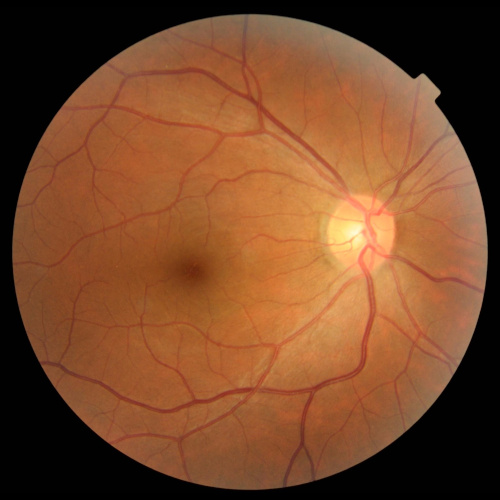
\includegraphics[width=0.3\textwidth]{images/TRAIN000004_cut.JPG}
 \caption{Imagem de fundo de olho. Obtida do banco de dados JustRAIGS.}
 \label{fig:fundus}
\end{figure}

\begin{comment}
Dentre as características observadas estão: 1, 2, 3, 4 e 5. cite{"Five rules to evaluate the optic disc and retinal nerve fiber layer for glaucoma"}

A capacidade da inteligência artificial em --- atrai seu uso na medicina. cite{alguem}

uso de IA com imagens médicas aumentou\\


fazer a avaliação manual gera divergência entre médicos, falta de padronização -> podemos fazer de forma automática
\end{comment}

\begin{comment}
da pra falar que médicas acreditam no potencial da IA
tem essa pesquisa aqui mas me parece muito restrita: só australia e nova zelancia e só com  trainees
...médicos acreditam que IA vai melhorar o trabalho deles... \cite{scheetz_survey_2021}
\end{comment}

Recentemente, diversas técnicas de aprendizagem profunda vem sendo aplicadas no diagnóstico de doenças com base em imagens de fundo de olho, inclusive para o glaucoma~\cite{li_review_2021}. Para possibilitar o desenvolvimento desses modelos, bancos de dados com imagens de fundo de olho classificadas por oftalmologistas foram criados e alguns deles disponibilizados publicamente, como o RIGA~\cite{riga}, ORIGA~\cite{origa}, RIM-ONE DL~\cite{RIMONEDL} e JustRAIGS~\cite{justraigs}. Um quadro resumo com alguns conjuntos de dados é apresentado na Tabela~\ref{tab:datasets}. 

\begin{figure}[htb]
 \centering
 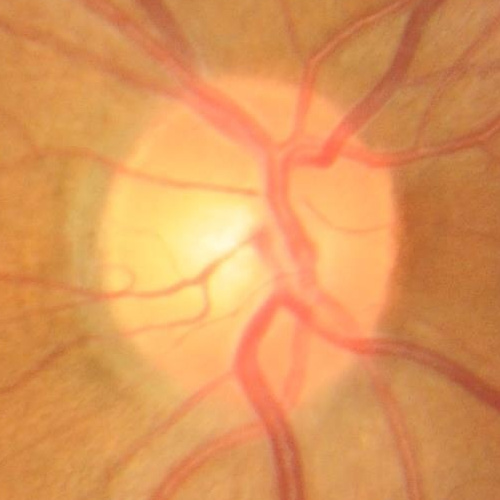
\includegraphics[width=0.3\textwidth]{images/disk.jpg}
 \caption{Disco ótico em destaque. Obtida do banco de dados JustRAIGS.}
 \label{fig:disk}
\end{figure}

Trabalhos anteriores conseguiram realizar a classificação de imagens entre glaucoma e não glaucoma utilizando diferentes técnicas. Noronha et al. (2014) utilizou cumulantes de alta ordem para identificar glaucoma em 272 imagens de fundo de olho obtidas por conta própria, obtendo acurácia de 84.72\%~\cite{noronha2014hoc}. Chen et al. (2015) implementou uma rede neural convolucional, contendo seis camadas sendo quatro convolucionais e 2 totalmente conectadas, e a treinou em dois bancos de dados privados, obtendo de resultado os valores de área sobre curva (AUC) 0.831 e 0.887~\cite{chen2015cnn}. Liu et al. (2019) desenvolveu uma rede convolucional baseada na arquitetura ResNet e a treinou com 241.032 imagens, obtendo uma AUC de 0.996~\cite{liu_cnn_2019}. Um quadro resumo com estes e outros trabalhos é apresentado na Tabela~\ref{tab:trabalhos}.

Em seu estudo de revisão, a respeito do uso de aprendizagem profunda em imagens de fundo de olho, Li et al.~\cite{li_review_2021} aponta como algumas das limitações e áreas para melhorias futuras a baixa disponibilidade de dados anotados com qualidade e a falta de interpretabilidade dos resultados, característica inerente à aprendizagem profunda.

%% CSS: citar alguns exemplos de anotações extra do justRaigs, para exemplificar
O banco de dados JustRAIGS, além de incluir anotações entre referenciável para glaucoma ou não para 101.422 imagens, também possui 10 anotações adicionais, para sinais observados pelos avaliadores, que justifiquem a escolha da imagem como referenciável para glaucoma, naquelas assim marcadas~\cite{justraigs_article}.

O presente trabalho procura explorar o uso de redes neurais convolucionais no problema de classificação do glaucoma em imagens de fundo olho, além de investigar o uso das anotações adicionais presentes no JustRAIGS como forma de auxiliar na interpretabilidade dos resultados produzidos pelos modelos.

O restante do texto é organizado da seguinte maneira: em primeiro lugar, apresentamos os objetivos deste trabalho na Seção~\ref{sec:objetivo}. A Seção~\ref{sec:methodology} explora o conjunto de dados escolhido, descreve o desenvolvimento e resultados do segmentador do disco ótico e descreve o treinamento do classificador preliminar. Seguindo na Seção~\ref{sec:results}, apresentamos os resultados por ele obtidos. Por fim, as conclusões são apresentadas na Seção~\ref{sec:conclusions}, junto com o plano de trabalho proposto para a próxima etapa do trabalho (Seção~\ref{sec:schedule}).

\begin{comment}
DESCONSIDERAR ESSE BLOCO

usando redes neurais\\
e até mesmo técnicas de processamento de sinais\cite{Noronha2014}

porem:
\begin{itemize}
 \item datasets limitados (agora temos um de 100k imagens) e alguns são privados
 \item falta de justificativa, blackbox ~\cite{li_review_2021} 7.2.5, usar features adicionais para explicar decisão
\end{itemize}

suposições que precisam ser sustentadas:\\
1- razão OD e OC é a melhor forma de identificar glaucoma\\
2- CNN é melhor de que calcular a razão ente OD e OC: [Chen, 2015] afirma mas não sustenta. Cita [3]\\

2) Diaz-Pinto, 2019: usando CNN não precisa fazer segmentação perfeita do OD e do OC
"Important limitations of the methods that are based on handcrafted characteristics (CDR, Area Cup/Disc ratio (ACDR), vessel kinks and ISNT rule) is the significant disagreement in estimating them even between expert human graders. For that reason, new algorithms have been focused on automatic feature extraction such as the data-driven methods [3] and convolutional neural networks (CNNs)."\\
Menciona alguns trabalhos que foram pela abordagem da segmentação e os resultados obtidos.

investigar:
Chen, 2015: 17 5 6 14, 2, 12, 13\\
Noronha, 2014: 9, 16, 17, 18

\end{comment}

\begin{table}[htb]
    \centering
    \begin{tabular}{|c|c|c|}
    \hline
    Nome & Nº de imagens & Ano de publicação \\
    \hline
    ORIGA & 650 & 2010 \\
    \hline
    DRISHTI-GS1 & 101 & 2015 \\
    \hline
    RIGA & 750 & 2018 \\
    \hline
    RIM-ONE DL & 485 & 2020 \\
    \hline
    REFUGE & 1200 & 2020 \\
    \hline
    JustRAIGS & 101.442 & 2024 \\
    \hline
    \end{tabular}
    \caption{Bancos de dados para avaliação de glaucoma}
    \label{tab:datasets}
\end{table}

\begin{table}[htb]
    \centering
    % o formato p (de parágrafo) permite ajustar largura e causa quebra de linha
    \begin{tabular}{|l|l|p{3cm}|c|c|}
    \hline
    Artigo                                      & Método      & Banco de dados                 & ACC   & AUC   \\
    \hline
    Noronha et al. (2014)~\cite{noronha2014hoc} & Cumulantes  & Privado com 272 imagens        & 0.847 &  -    \\
    \hline
    Chen et al. (2015)~\cite{chen2015cnn}       & CNN própria & ORIGA                          & -     & 0.831 \\
    \hline
    Chen et al. (2015)~\cite{chen2015cnn}       & CNN própria & ORIGA, SCES                    & -     & 0.887 \\
    \hline
    Ferreira et al. (2018)~\cite{ferreira_cnn_2018} & U-Net   & RIM-ONE, DRISHTI-GS, DRIONS-DB & 1     & 1     \\
    \hline
    Liu et al. (2019)~\cite{liu_cnn_2019}       & ResNet      & Privado com 241.032 imagens    & 0.996 & -     \\
    \hline
    Nawaz et al. (2022)~\cite{nawaz_efficient_2022} & EfficientNet-B0 & ORIGA                  & 0.972 & 0.979 \\
    \hline
    \end{tabular}
    \caption{Trabalhos anteriores e resultados obtidos}
    \label{tab:trabalhos}
\end{table}

\bigskip

\section{Objetivos}
\label{sec:objetivo}

\begin{comment}
Objetivos: (devem ser mensuráveis, chegar no final do trabalho e dizer que atingiu)
  criar modelo que seja interpretável
secundário:
 - "comparar modelos quanto à interpretabilidade"
 - determinar metodologia para comparar interpretabilidade
\end{comment}

O objetivo geral deste trabalho é realizar a identificação de glaucoma em imagens de fundo de olho, utilizando um modelo de aprendizagem profunda, que seja interpretável.

Os objetivos específicos são:
\begin{itemize}
 \item realizar a segmentação do disco ótico, a região de interesse (ROI)
 % revisão da literatura sobre diferentes arquiteturas de forma a organizar conhecimento
\end{itemize}

\bigskip


\bigskip

\section{Materiais e Métodos}
\label{sec:methodology}

%% CSS: Escrever um parágrafo introdutório delineando a estrutura da seção
Nesta seção, descrevemos as características do conjunto de dados e os tratamentos nele feitos, os passos realizados para a construção de um segmentador da região de interesse e os resultados obtidos, e os procedimentos e técnicas adotados para o treinamento de um classificador preliminar.

\subsection{Conjunto de dados}
\label{sec:dataset}

Foi escolhido o conjunto de dados JustRAIGS~\cite{justraigs} que contém 101.442 imagens de fundo de olho publicamente disponíveis, derivado do conjunto de dados REGAIS – \emph{Rotterdam EyePACS Glaucoma AI Screening}~\cite{justraigs_article}. As imagens foram providas pelo EyePACS LLC em Santa Cruz, Califórnia nos EUA enquanto as anotações foram providas pelo Instituto de Oftalmologia de Roterdã (\emph{Rotterdam Ophthalmic Institute}) do \emph{Rotterdam Eye Hospital} em Roterdã nos Países Baixos.

%% CSS: repita a referência para o artigo, como mudou de parágrafo, pode gerar dúvida
%% LZT: apenas no final, ou entre cada frase? coloquei no final
Cada imagem foi anotada por dois avaliadores (A1 e A2), selecionados aleatoriamente dentre um conjunto de avaliadores qualificados. 
Para cada imagem, o avaliador deveria escolher uma classificação principal entre referenciável para glaucoma (referable glaucoma - RG), não referenciável (no referable glaucoma - NRG) ou ainda se não era possível avaliar a imagem (ungradable - U). Referenciável para glaucoma deveria ser escolhido se fossem esperadas perdas no campo de visão para o olho avaliado.
Caso os dois avaliadores concordassem na classificação principal, essa classificação era dada como final, caso contrário, um terceiro avaliador (A3), especialista em glaucoma, anotava a imagem e essa anotação era dada como final.~\cite{justraigs_article}

Para os casos em que o avaliador julgasse como referenciável para glaucoma, ele poderia selecionar até 10 anotação adicionais, que representam características aparentes de um olho com glaucoma, de forma a justificar sua escolha. \cite{justraigs_article}

As anotações adicionais são:
\begin{itemize}
    \item \textbf{ANRS}: Aparência do anel neurorretiniano superior (\emph{Appearance neuroretinal rim superiorly})
    \item \textbf{ANRI}: Aparência do anel neurorretiniano inferior (\emph{Appearance neuroretinal rim inferiorly})
    \item \textbf{RNFLDS}: Defeito na camada de fibras nervosas da retina superior (\emph{Retinal nerve fiber layer defect superiorly})
    \item \textbf{RNFLDI}: Defeito na camada de fibras nervosas da retina inferior (\emph{Retinal nerve fiber layer defect inferiorly})
    \item \textbf{BCLVS}: Exposição de vasos circunlineares superior (\emph{Baring circumlinear vessel superiorly})
    \item \textbf{BCLVI}: Exposição de vasos circunlineares inferior (\emph{Baring circumlinear vessel inferiorly})
    \item \textbf{NVT}: Nasalização do tronco vascular (\emph{Nasalisation of vessel trunk})
    \item \textbf{DH}: Hemorragias do disco óptico (\emph{Disc hemorrhages})
    \item \textbf{LD}: Pontos laminares (\emph{Laminar dots})
    \item \textbf{LC}: Escavação aumentada (\emph{Large cup})
\end{itemize}

Discordâncias nessas anotações adicionais, contudo, não foram resolvidas. Isto significa que há casos em que, apesar de A1 e A2 terem concordado na classificação principal como glaucoma, eles podem ter selecionado anotações adicionais diferentes para justificar sua escolha e, nesses casos, A3 não foi requisitado. Sendo assim, o conjunto de dados inclui a anotação principal final e as anotações principal e adicionais de cada avaliador. Imagens cuja classificação final foi U não foram incluídas no JustRAIGS.

Para obter um valor final às anotações adicionais, no escopo deste trabalho, adotamos a seguinte regra para a resolução:

\begin{itemize}
    \item A1 e A2 concordam na anotação principal $\rightarrow$ para cada anotação adicional, valor final é 1 se A1 e A2 marcaram como 1, do contrário 0
    \item A1 concorda com A3 $\rightarrow$ aplicamos a regra acima para os valores de A1 e A3
    \item A2 concorda com A3 $\rightarrow$ aplicamos a regra para os valores de A2 e A3
    \item todos discordam $\rightarrow$ usamos os valores de A3
\end{itemize}

% RESUMO
% A1 e A2 concordam na principal -> interseção entre A1 e A2
% A1 e A3 concordam -> interseção entre A1 e A3
% A2 e A3 concordam -> interseção entre A2 e A3
% todos discordam (NRG, U, RG) -> A3

As análises e desenvolvimentos que seguem são baseadas no resultado obtido por meio desta regra.

\subsubsection{Análise}
\label{sec:dataset:analysis}
Das 101.442 imagens que o conjunto de dados alega possuir, 19 não foram encontradas, restando 101.423. O conjunto é bastante desbalanceado: dentre todas as imagens, apenas 3.270 receberam anotação final para glaucoma, o que representa aproximadamente 3,22\% ou 1 em cada 31.

Das anotações adicionais, ANRI é a mais frequente, aparecendo em 69,08\% dos casos referenciáveis para glaucoma (ou 2,23\% do total), DH por sua vez é a menos frequente, aparecendo em apenas 2,45\% (0,08\%). É possível observar certas correlações entre as anotações adicionais, apresentadas na Figura~\ref{fig:labels_correlation} por meio de uma matriz de correlação.

\begin{figure}[htb]
 \centering
 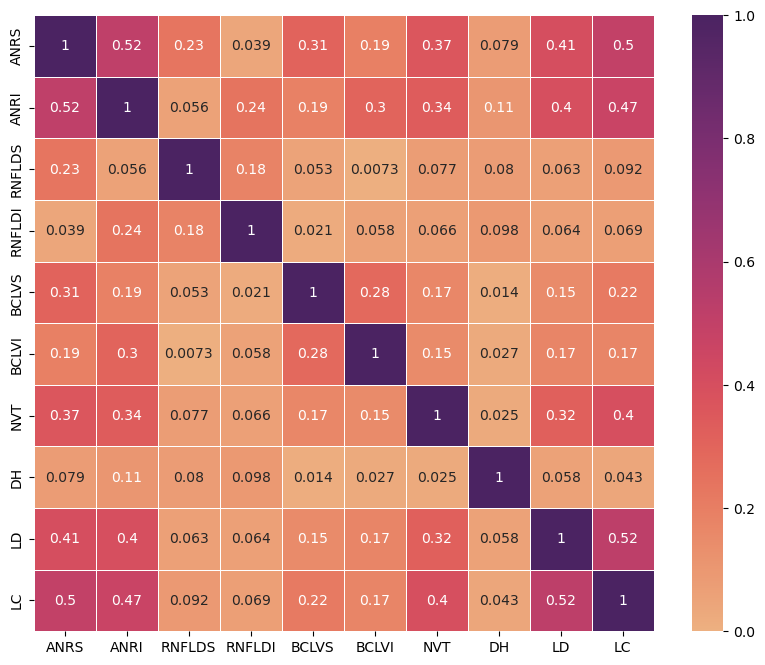
\includegraphics[width=0.7\textwidth]{images/correlation.png}
 \caption{Matriz de correlação entre anotações adicionais}
 \label{fig:labels_correlation}
\end{figure}

\subsubsection{Imagens}
\label{sec:dataset:images}

A aquisição das imagens foi feita em vários centros de triagem com câmeras diferentes \cite{justraigs_article}.
É possível observar grande variação de brilho, contraste e nitidez nas imagens do conjunto de dados, como ilustrado na Figura~\ref{fig:images_variations_1}.

\begin{figure}
    \centering
    \begin{subfigure}[b]{0.2\textwidth}
        \centering
        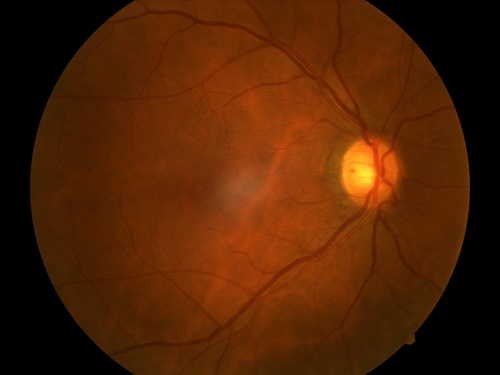
\includegraphics[width=\textwidth]{images/examples_from_dataset/TRAIN000282.JPG}
        \label{fig:images_variations_1_1}
    \end{subfigure}
    \hfill
    \begin{subfigure}[b]{0.2\textwidth}
        \centering
        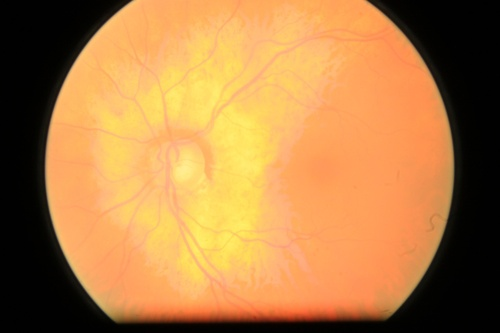
\includegraphics[width=\textwidth]{images/examples_from_dataset/TRAIN012425.JPG}
        \label{fig:images_variations_1_2}
    \end{subfigure}
    \hfill
    \begin{subfigure}[b]{0.2\textwidth}
        \centering
        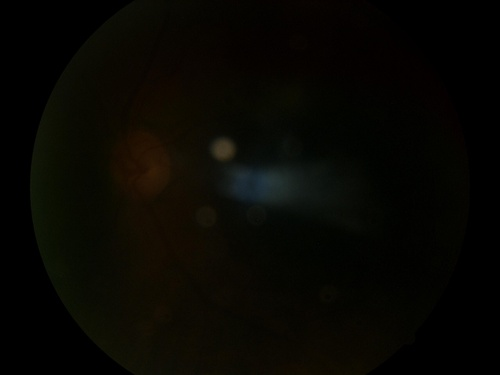
\includegraphics[width=\textwidth]{images/examples_from_dataset/TRAIN013211.JPG}
        \label{fig:images_variations_1_3}
    \end{subfigure}
    \hfill
    \begin{subfigure}[b]{0.2\textwidth}
        \centering
        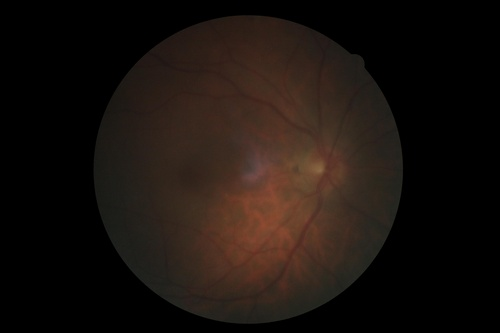
\includegraphics[width=\textwidth]{images/examples_from_dataset/TRAIN061871.JPG}
        \label{fig:images_variations_1_4}
    \end{subfigure}
    \caption{Variações de luminosidade e contraste entre imagens do JustRAIGS}
    \label{fig:images_variations_1}
\end{figure}

Nota-se também a presença de artefatos de aquisição variados em parte das imagens, como mostrado na Figura~\ref{fig:images_variations_2}.

\begin{figure}
    \centering
    \begin{subfigure}[b]{0.2\textwidth}
        \centering
        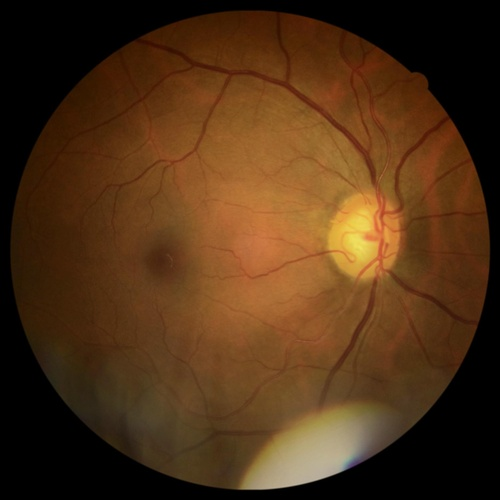
\includegraphics[width=\textwidth]{images/examples_from_dataset/TRAIN025848.JPG}
        \label{fig:images_variations_2_1}
    \end{subfigure}
    \hfill
    \begin{subfigure}[b]{0.2\textwidth}
        \centering
        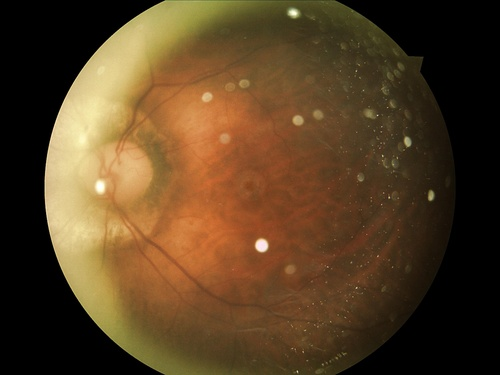
\includegraphics[width=\textwidth]{images/examples_from_dataset/TRAIN045963.JPG}
        \label{fig:images_variations_2_2}
    \end{subfigure}
    \hfill
    \begin{subfigure}[b]{0.2\textwidth}
        \centering
        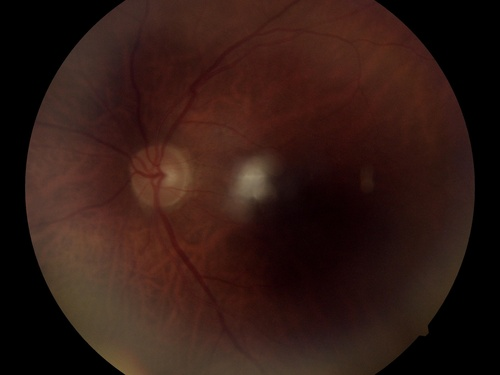
\includegraphics[width=\textwidth]{images/examples_from_dataset/TRAIN049428.JPG}
        \label{fig:images_variations_2_3}
    \end{subfigure}
    \hfill
    \begin{subfigure}[b]{0.2\textwidth}
        \centering
        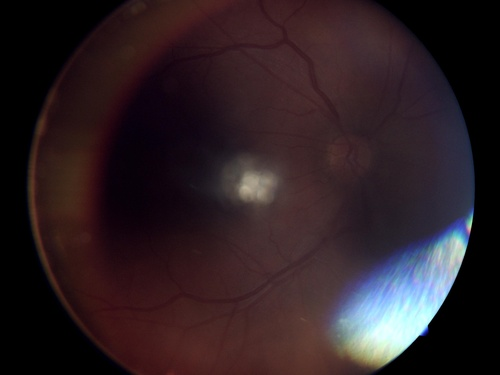
\includegraphics[width=\textwidth]{images/examples_from_dataset/TRAIN065536.JPG}
        \label{fig:images_variations_2_4}
    \end{subfigure}
    \caption{Imagens com artefatos de aquisição variados}
    \label{fig:images_variations_2}
\end{figure}

\subsubsection{Divisão entre treino e teste}
\label{sec:dataset:split}

O conjunto de dados foi dividido na proporção 80\% para treinamento e 20\% para teste. Para realizar essa divisão, o conjunto foi inicialmente dividido entre NRG e RG. Para a porção de NRG foi feita uma divisão aleatória comum. Já para a porção de RG, com o intuito de preservar a proporção das anotações adicionais, foi feita uma amostragem estratificada utilizando a classe \emph{StratifiedShuffleSplit} e o método \emph{split} da biblioteca \emph{scikit-learn}. Devido a grande quantidade de anotações adicionais (10), não foi possível utilizar todas elas para a amostragem. No lugar, todas as possíveis permutações de 2, 3, 4 e 5 das anotações adicionais foram testadas. O uso de mais de 6 se mostrou impraticável devido à exaustão de representantes por classe. Para escolher a melhor permutação de anotações adicionais, foi utilizada uma métrica que avaliava a qualidade da divisão. A métrica se baseou na soma dos quadrados da diferença entre a proporção obtida e desejada para cada anotação entre os dois conjuntos. Quanto menor a pontuação, mais balanceada e representativa era a divisão. Essa abordagem garantiu que a representatividade das anotações adicionais fosse preservada entre os conjuntos, mesmo para classes com baixa ocorrência.

\subsection{Segmentação da região de interesse}
\label{sec:segmentation}

%% LZT: missing citation
As características visuais associadas ao glaucoma, no exame de fundo de olho, estão ou no disco ótico ou em seu entorno. Portanto, para melhor aproveitamento da rede neural classificadora, segmentamos as imagens na região do disco.

Para realizar essa segmentação, foi utilizado um modelo de aprendizagem profunda chamado Ultralytics YOLO11, capaz de realizar múltiplas tarefas de visão computacional em tempo real, como detecção de objetos, segmentação, classificação ou estimativa de pose humana. Ele pode ser treinado em novas bases de dados para aplicações específicas. Para cada tarefa existe uma família de modelos com quantidades de parâmetros diferentes \cite{YOLO_2023}. Escolhemos o modelo \emph{yolo11m} para detecção de objetos.

Para treinar o YOLO, foram aleatoriamente selecionadas 1400 imagens do conjunto de treinamento: 1000 para treino, 200 para validação e 200 para teste. Em cada um dos conjuntos a proporção de RG foi de 20\%. Para cada imagem, o disco ótico foi manualmente anotado por meio de uma caixa delimitadora com duas coordenadas. As anotações foram feitas com o software AnyLabeling \cite{anylabeling}.

\begin{figure}[htb]
 \centering
 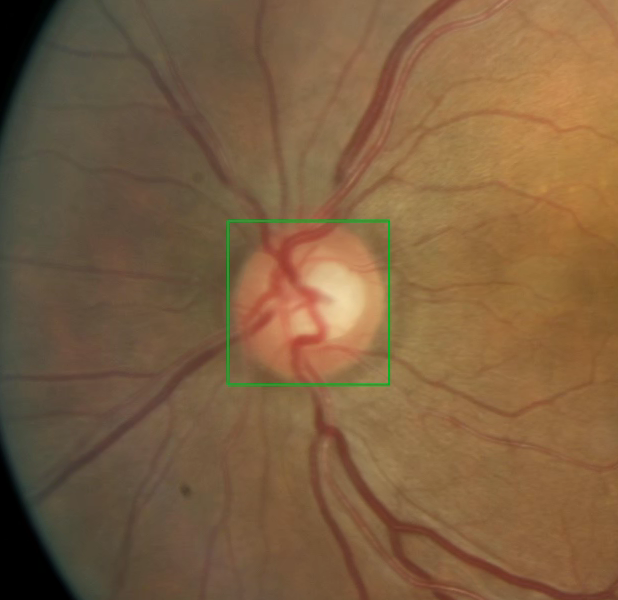
\includegraphics[width=0.3\textwidth]{images/disk_labeling.png}
 \caption{Disco ótico anotado no software AnyLabeling. Imagem original obtida do banco de dados JustRAIGS.}
 \label{fig:disk_labeling}
\end{figure}

%% CSS: criar um glossário das métricas
Foi feito o treinamento do segmentador com 100 épocas utilizando os parâmetros padrões do YOLO. Após o treinamento, no conjunto de validação o modelo atingiu precisão e recall 1, mAP50 0.995 e mAP50-95 0.945. No teste, apresentou precisão 0.995, recall 1, mAP50 0.995 e mAP50-95 0.936.

%% CSS: reescrever para deixar mais claro, pode dar a impressão que você está afirmando que algumas imagens têm dois discos ópticos.
Em seguida, o segmentador foi aplicado para todo o conjunto de treinamento definido anteriormente na Seção~\ref{sec:dataset:split}. Das 81.138 imagens, em 80.725 (99.49\%) foi identificado apenas um disco ótico, em 332 (0.41\%) mais de um e em 81 (0.10\%) nenhum. Para todas as detecções, utilizamos o \emph{score} mínimo de 0.25, valor padrão do YOLO.

Analisando as 81 imagens em que nenhuma detecção foi retornada, não conseguimos identificar uma causa predominante para a ausência de detecções. Listamos algumas das características dessas imagens, que se manifestam de formas variadas:

\begin{itemize}
    \item disco ótico com limites pouco definidos
    \item imagens com baixo contraste em que disco ótico aparece "apagado"
    \item imagens desfocadas ou com baixa nitidez
    \item lesões ou deformações anatômicas diversas ao redor do disco ótico
\end{itemize}

Alguns exemplos são apresentados na Figura~\ref{fig:images_no_box}.

\begin{figure}
    \centering
    \begin{subfigure}[b]{0.47\textwidth}
        \centering
        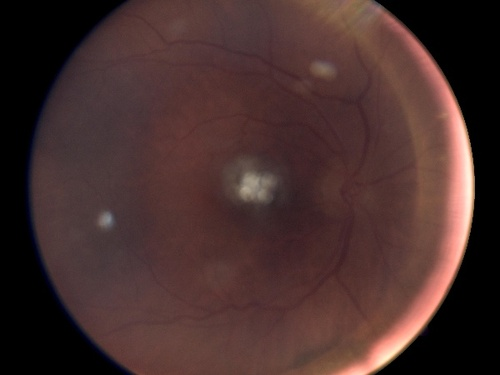
\includegraphics[width=\textwidth]{images/no_box/TRAIN000883_boxes.jpg}
        \label{fig:images_no_box_1}
    \end{subfigure}
    \hfill
    \begin{subfigure}[b]{0.47\textwidth}
        \centering
        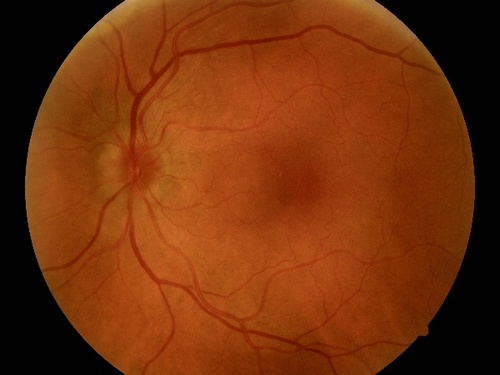
\includegraphics[width=\textwidth]{images/no_box/TRAIN045856_boxes.jpg}
        \label{fig:images_no_box_2}
    \end{subfigure}
    \break
    \begin{subfigure}[b]{0.47\textwidth}
        \centering
        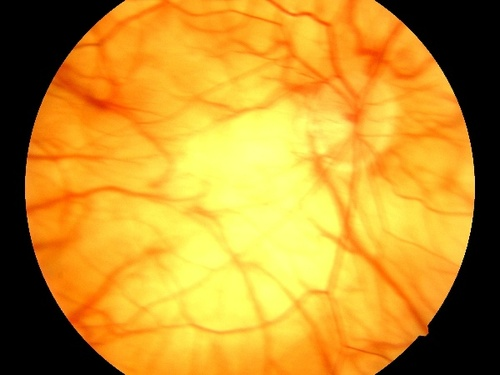
\includegraphics[width=\textwidth]{images/no_box/TRAIN046833_boxes.jpg}
        \label{fig:images_no_box_3}
    \end{subfigure}
    \hfill
    \begin{subfigure}[b]{0.47\textwidth}
        \centering
        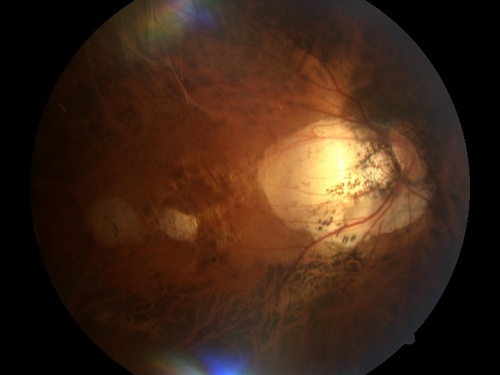
\includegraphics[width=\textwidth]{images/no_box/TRAIN099284_boxes.jpg}
        \label{fig:images_no_box_4}
    \end{subfigure}
    \caption{Imagens sem detecção pelo YOLO}
    \label{fig:images_no_box}
\end{figure}

Por outro lado, analisando as 332 imagens para as quais o modelo retornou mais de uma predição, identificamos alguns artefatos de aquisição predominantes que confundiram o modelo. Algumas imagens com múltiplas detecções são apresentados na Figura~\ref{fig:multiple_boxes}.

\begin{figure}
    \centering
    \begin{subfigure}[b]{0.47\textwidth}
        \centering
        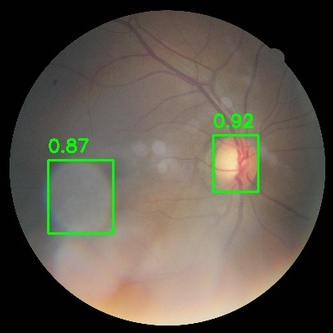
\includegraphics[width=\textwidth]{images/multiple_boxes/TRAIN003802_boxes.jpg}
        \label{fig:multiple_boxes_1}
    \end{subfigure}
    \hfill
    \begin{subfigure}[b]{0.47\textwidth}
        \centering
        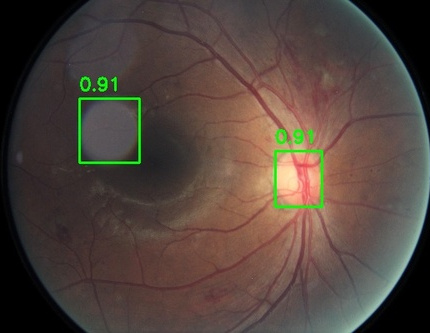
\includegraphics[width=\textwidth]{images/multiple_boxes/TRAIN031744_boxes.jpg}
        \label{fig:multiple_boxes_2}
    \end{subfigure}
    \break
    \begin{subfigure}[b]{0.47\textwidth}
        \centering
        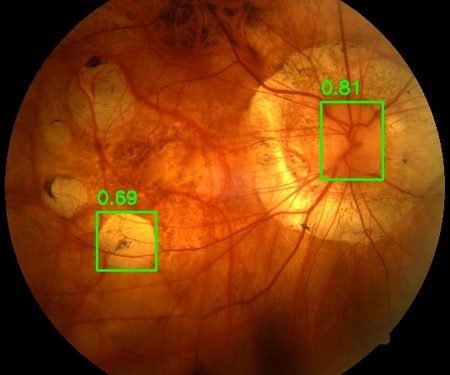
\includegraphics[width=\textwidth]{images/multiple_boxes/TRAIN011494_boxes.jpg}
        \label{fig:multiple_boxes_3}
    \end{subfigure}
    \hfill
    \begin{subfigure}[b]{0.47\textwidth}
        \centering
        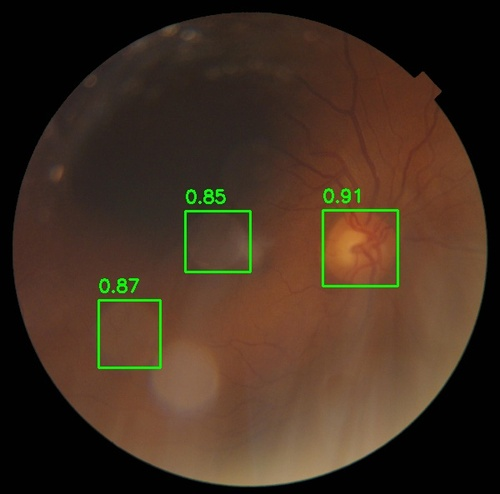
\includegraphics[width=\textwidth]{images/multiple_boxes/TRAIN031299_boxes.jpg}
        \label{fig:multiple_boxes_4}
    \end{subfigure}
    \caption{Imagens com múltiplas detecções pelo YOLO e score atribuído}
    \label{fig:multiple_boxes}
\end{figure}

Resolvemos então escolher aleatoriamente 100 imagens dentre as 332 para treinar um novo segmentador. Foram anotadas manualmente e incluídas no conjunto de dados usado anteriormente, 50, 25 e 25 imagens para treino, validação e teste, respectivamente. Um novo treinamento foi feito então, utilizando os mesmos parâmetros do anterior. Devido à falta de experiência, adotamos uma postura cautelosa em não anotar as imagens para as quais o modelo não retornou nenhum resultado. Em uma aplicação real, casos como estes seriam encaminhados para avaliação de um médico. 

Desta vez, na validação o modelo atingiu presisão e recall 1, mAP50 0.995 e mAP50-95 0.944, enquanto que no teste atingiu precisão 0.999, recall 0.991 mAP50 0.995 e mAP50-95 0.934.

Ao aplicar a segunda geração em todo o conjunto de treino, desta vez, o modelo identificou apenas um disco ótico em 81.016 imagens (99.85\%), mais de um em 63 (0.08\%) e nenhum em 59 (0.07\%).

% IMAGENS USADAS NO YOLO
%       gen1  new  gen2
% total 1400  100  1500
% train 1000   50  1050
% val    200   25   225
% test   200   25   225

\subsection{Classificação}
\label{sec:classification}

Antes de serem utilizadas no classificador, todas as imagens foram cortadas no entorno do disco ótico detectado pelo segmentador. A região do corte foi definida com as coordenadas retornadas, adicionadas de uma margem de 50\% para cada eixo.

Com o objetivo de contornar o desbalanceamento entre as classes NRG e RG durante o treinamento, todas as 2.610 imagens RG disponíveis no conjunto de treinamento foram espelhadas horizontalmente e salvas como novas imagens. Além disso, apenas um subconjunto de 10 mil imagens NRG aleatoriamente selecionadas foi utilizado, totalizando portanto 15.220 imagens.

% IMAGENS USADAS NO CLASSIFICADOR
% NRG   10.000
% RG     5.220 (2.610 x 2)
% total 15.220

Para a tarefa de classificação entre NRG e RG, foi treinada uma ResNet50, por meio da técnica de transferência de aprendizagem, pré-treinada no conjunto de dados ImageNet. Removemos a camada superior e adicionamos uma camada GlobalAveragePooling2D, duas camadas totalmente conectadas de tamanhos 1024 e 256 com função de ativação ReLU e uma camada totalmente conectada de saída de tamanho 1 com função sigmoide. Entre as novas camadas, foi aplicado \emph{dropout} com taxa de 50\%.

Durante o treinamento, o conjunto de dados descrito foi dividido em 80\% para treinamento e 20\% para validação, e foi aumentado artificialmente com operações aleatórias de translação, rotação e zoom. Numa primeira etapa, as camadas originais da ResNet50 foram congeladas e realizado o treinamento apenas das camadas superiores novas. Em seguida, todas as camadas foram treinadas a uma taxa de aprendizagem menor, etapa chamada de ajuste fino (\emph{fine-tuning}).

As duas etapas fizeram uso da técnica de parada antecipada (\emph{early stopping}), observando a área da curva precisão-recall do conjunto de validação.

Foram feitos experimentos com os otimizadores \emph{RMSprop} e \emph{ADAM}, com taxa de aprendizagem de $10\textsuperscript{-4}$ na primeira etapa e $10\textsuperscript{-5}$ no ajuste fino, e função de perda entropia cruzada binária (\emph{binary crossentropy}).

\subsection{Recursos computacionais}
\label{sec:resources}

Todos os modelos foram implementados em Python com Keras utilizando o TensorFlow v2.18.0 de backend, com exceção do YOLO (Ultralytics) que utiliza o PyTorch. As versões dos pacotes eram: Python 3.10.12, Keras 3.6.0, TensorFlow 2.18.0, Ultralytics 8.3.18.
Os códigos foram executados com o sistema operacional Pop!\_OS 22.04, kernel Linux 6.9.3, contendo instalado o driver da NVIDIA 560.35.03 e as bibliotecas NVIDIA CUDA 12.6 e NVIDIA cuDNN 9.5.1.
O computador estava equipado com um processador Intel i7-10700K, 32 GB de RAM e uma GPU NVIDIA GeForce RTX 3070.

\section{Resultados}
\label{sec:results}

% LZT: qual métrica usar para escolher o melhor modelo?
%      adotado prc, mesmo usado no early-stopping

O melhor resultado foi obtido no experimento que utilizou o otimizador ADAM. No conjunto de validação, o modelo atingiu AUC-ROC 0,9789, PRC 0,9503, F1 0,9180, precisão 0,9060 e recall 0,9304. Foram necessárias 92 epochs na primeira etapa e 33 epochs na etapa de ajuste fino. A Figura~\ref{fig:gen2_005_tt_metrics} apresenta as métricas durante a primeira fase, a Figura~\ref{fig:gen2_005_ft_metrics} métricas do ajuste fino e na Figura~\ref{fig:gen2_005_confusion_matrix} apresentamos a matriz de confusão.

\begin{figure}[ht]
 \centering
 \includegraphics[width=1.0\textwidth]{images/gen2_005/top_training_metrics.png}
 \caption{Métricas da primeira etapa de treinamento do classificador}
 \label{fig:gen2_005_tt_metrics}
\end{figure}

\begin{figure}[h!t]
 \centering
 \includegraphics[width=1.0\textwidth]{images/gen2_005/fine_tuning_metrics.png}
 \caption{Métricas da etapa de ajuste fino do classificador}
 \label{fig:gen2_005_ft_metrics}
\end{figure}

\begin{figure}[htb]
 \centering
 \includegraphics[width=0.6\textwidth]{images/gen2_005/conf.png}
 \caption{Matriz de confusão do classificador}
 \label{fig:gen2_005_confusion_matrix}
\end{figure}

\section{Conclusões e Trabalhos Futuros}
\label{sec:conclusions}

Neste trabalho foi apresentado um modelo capaz de detectar o disco ótico em imagens de fundo de olho, que obteve precisão 0.999, recall 0.991 mAP50 0.995 e mAP50-95 0.934.

Destacamos o impacto positivo em se fazer uma curadoria adicional no conjunto de dados, em busca de casos difíceis para incluí-los no treinamento do modelo. Tal abordagem possibilitou reduzir o número de ambiguidades, apesar da ligeira queda de desempenho no teste. Essa queda pode ser justificada pela inclusão super representada de casos mais difíceis.

Também apresentamos um classificador preliminar obtido do treinamento de uma CNN da arquitetura ResNet50, por meio de transferência de aprendizagem, capaz de identificar glaucoma em imagens de fundo de olho. O modelo apresentou uma performance ligeiramente abaixo de trabalhos relacionados, mas é esperado que haja uma melhora com o uso de outras técnicas de aumentação de dados, normalização dos dados de entrada e melhor aproveitamento do conjunto de dados.

% LZT: devemos mover o plano de trabalho para o final? Ele menciona refinir
% o classificador que ainda nem foi apresentado
\subsection{Plano de trabalho}
\label{sec:schedule}

O plano de trabalho proposto, para o último de três períodos, contém as seguintes etapas:
\begin{itemize}
    \item \textbf{Refinar classificador:} continuar o treinamento do classificador, explorando outras técnicas de aumentação de dados, normalização dos dados de entrada e melhor aproveitamento do conjunto de dados
    \item \textbf{Avaliar e comparar classificador:} comparar a performance do classificador com outras publicações
    \item \textbf{Implementar classificador orientado a protótipos:} fazer adaptação de outros trabalhos que utilizam a ideia de protótipos para explorar a interpretabilidade
    \item \textbf{Revisão de fundamentos:} estudo e revisão de fundamentos teóricos
    \item \textbf{Escrita do relatório}
\end{itemize}

%% CSS: use letra maiúscula (Figura) quando referenciar uma figura específica do texto.
A Figura~\ref{fig:crono} apresenta o cronograma proposto com as etapas definidas acima.

\begin{figure}[htb]
 \centering
 \includegraphics[width=1.0\textwidth]{images/crono_q3.png}
 \caption{Cronograma de execução da proposta}
 \label{fig:crono}
\end{figure}


\bigskip

%% LZT: Como fazer para não incluir a lista completa de nomes? [SBB+21] ficou muito grande
%% CSS: Parte da mudança para biblatex; suspendendo por enquanto,
% ver comentário no preâmbulo (5/9/2024)
% \printbibliography
\bibliographystyle{alpha}%{hapalike}
\bibliography{ref.bib}


\end{document}
